\section{Ejercicio 6}


Los Latches y los flip-flops son elementos utilizados en el alamcenaje de información. Cada uno puede guardar un bit de información. La diferencia principal entre ellos es que el latch chequea continuamente la entrada, cambiando la salida en caso de alguna variaci\'on en la entrada. Por otro lado, el flip-flop puede pensarse como la integración de un latch y un cicruito que responde a un clock, cambiando la salida no solo cuando la entrada varía, sino cuando incide un flanco del clock. En otras palabras, los latches son circuitos asincrónicos mientras que los flip-flops son circuitos sincrónicos. En general un flip-flop está compuesto por muchas más compuertas lógicas que un latch, por ende se esperaría que los tiempos de respuesta sean distintos. 



\subsection{Latch SR}

Un tipo común de latches es el latch $SR$, por set-reset. Su circuito es el siguiente:

\begin{figure}[H]
	\centering
	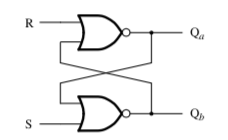
\includegraphics[width=0.5\textwidth]{Ejercicio6/Recursos/latchSR}
	\caption{Latch SR}
\end{figure}

Su tabla de verdad es como sigue:


\subsection{Flip-flop D}
Un tipo de flip-flop es el flip-flop tipo D, cuya salida copia la entrada $D$ cuando llegue un flanco de clock (puede configurarse el circuito para que sea ascendente o descendente). 

\begin{figure}[H]
	\centering
	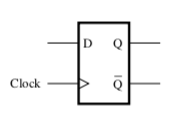
\includegraphics[width=0.5\textwidth]{Ejercicio6/Recursos/flipflopD}
	\caption{Flip-flop D}
\end{figure}

Un dispositivo de este estilo puede dividirse en dos partes, una que responde a cambios en el clock, y otra que almacena la información, en otras palabras un latch. El circuito siguiente es una configuración posible para la realización de un flip-flop tipo D:

\begin{figure}[H]
	\centering
	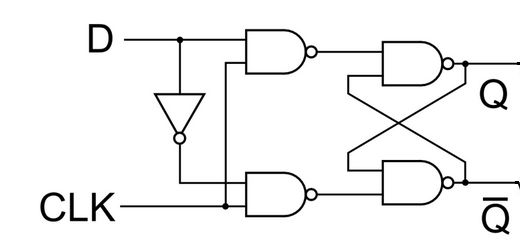
\includegraphics[width=0.6\textwidth]{Ejercicio6/Recursos/ffD_final}
	\caption{Gráfico flip-flop D}
\end{figure}


\subsection{Mediciones}
Para la medicion del Latch SR se alimentó el circuito con $5V_{DC}$ mientras que para el flip-flop se optó por una alimeatción igual a $10V_{DC}$. Todas las compuertas utilizadas son de tecnología CMOS. En la imagen que sigue pueden verse representadas la señal de clock (canal 1), la entrada (canal 2) y la salida del circuito (canal 3):

\begin{figure}[H]
	\centering
	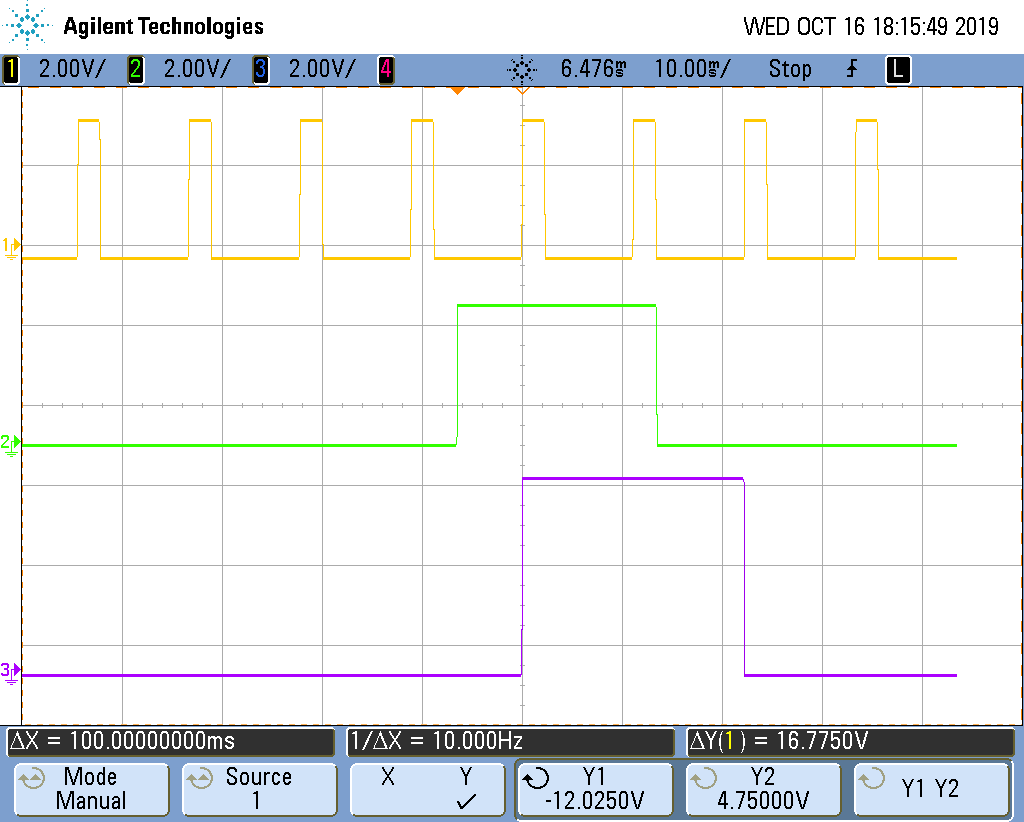
\includegraphics[width=0.9\textwidth]{Ejercicio6/Recursos/senales_ffD.png}
	\caption{Circuito flip-flop D}
\end{figure}

En el anterior diagrama, puede verse claramente el comportamiento del flip-flop tipo D. Recien cuando aparece un flanco positivo del reloj y la entrada al circuito es positiva también se observa un salida al circuito. Luego cuando la entrada baja a $0$, y nuevamente aparec un flanco de clock lo hace a su vez la salida. 

Uno de los parámetros que se midió es el tiempo de propagación desde el clock hasta la salida del circuito, en otras palabras cuanto tarda el circuito en reaccionar a una entrada. En la captura de osciloscopio se ve representado dicho tiempo:


\begin{figure}[H]
	\centering
	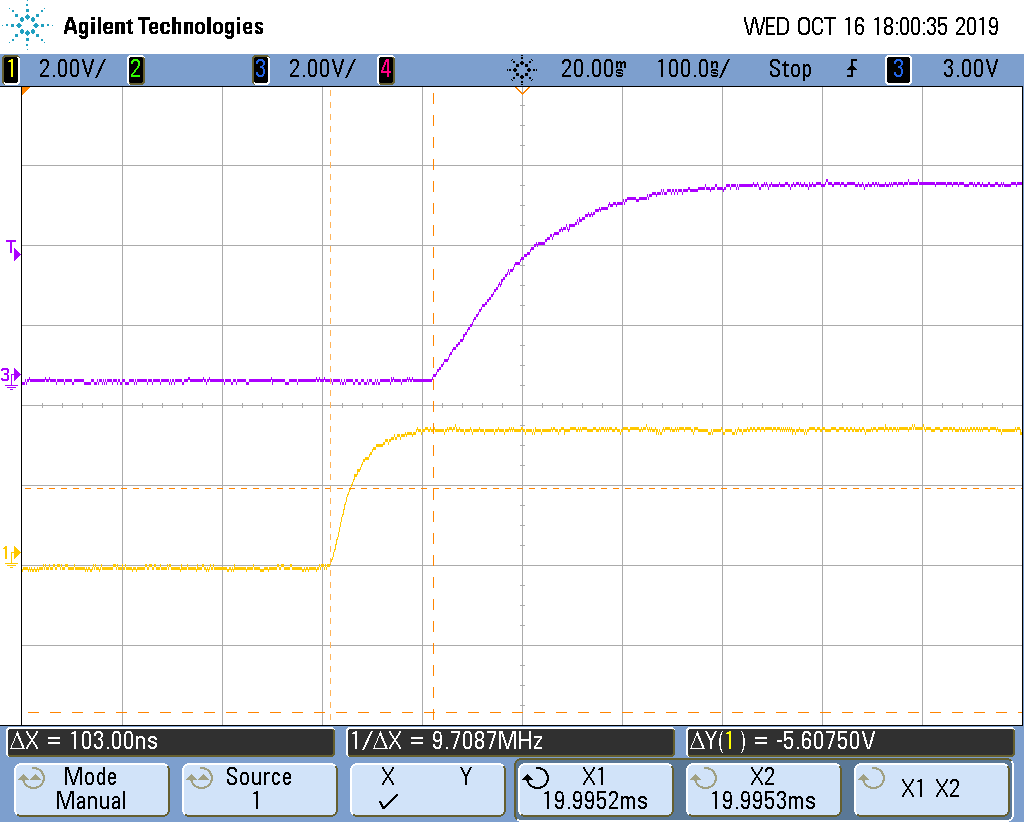
\includegraphics[width=0.9\textwidth]{Ejercicio6/Recursos/propagacion_ffD.png}
	\caption{Propagacion flip-flop D}
\end{figure}


En la siguiente tabla se resumen la totalidad de los resultados obtenidos, as\'i como los valores comerciales de comparaci\'on:

\begin{table}[H]
\begin{tabular}{llll}\hline
\multicolumn{1}{c}{}           & \multicolumn{1}{c}{Hold time (ns)} & \multicolumn{1}{c}{Set-up time (ns)} & Propagation Delay (ns) \\
\hline
Latch SR comercial (HC 373)    & 10                                 & 10                                   & 15-30                  \\
Latch SR implemenado           & 19                              &   17                                   &  44                \\
Flip-Flop D comercial (CD4013) & 2-5                                & 10-20                                & 65-130                 \\
Flip-Flop D implementado       & 8    &         17                             &             103           \\  \hline
\end{tabular}
\end{table}


En primer lugar, puede verse que para el caso del latch todos los tiempos medidos son superiores a los comerciales. No obstante, se está comparando respecto a un latch armado con compuertas NOR. UN mejor resultado puede lograrse armando el mismo circuito pero con compuertas NAND. Las compuertas NAND son prefreidas en general frente a las NOR debido a que consumen menos espacio, poseen menores corrientes de pérdida y fundamentalmente son más rápidas a las NOR. Lo anterior se debe a que para hacer una compuerta NOR de dos entrada se precisan 2 transistores PMOS en serie y dos transistorres NMOS en paralelo. Ahora bien, un requerimiento básico de de la tecnología CMOS es que el rise-time y el fall-time sean iguales. Para lograr lo anterior, en el caso de las NOR se agranda el tamaño del gate de los transistores PMOS hasta cuatro veces más que el de los NMOS. En el caso de las compuertas NAND los PMOS están en paralelo y los NMOS en serie, por ende el gate de los PMOS tiene que ser solamente dos veces más grande. En consecuencia las compuertas NAND son preferibles frente a las NOR. 



Realizando nuevamente el circuito con compuertas NAND, se lograron mejroes resultados: hold time igual a $15ns$, set-up time igual a $14ns$ y propagation delay igual a $32ns$. Las diferencias en este caso puede ser atribuidas a la integración de las compuertas en el circuito comercial. 



Por otro lado, los resultados para el flip-flop D son muy similares a los valores comerciales, el tiempo de propagación está incluso dentro del rango brindado por el fabricante. Además si se suma la propagación individual de cada compuerta NAND utilizada ($50ns$), se ve que el valor obtenido concuerda con el mismo. Para este caso debido a la utilización de compuertas NAND todos los tiempos son más cercanos a las soluciones de mercado. 